Recall the definition of the triply-randomized negative binomial beta (TNBBeta)
distribution introduced in \citep{lederman2026triplyrandomizednegativebinomialbeta}:
\begin{align*}
    \text{TNBBeta}(y; p, q, \varepsilon) &= \text{beta}(y; \varepsilon, \varepsilon)\left[\frac{1 - q}{y(1 - y)}\gamma(y, p)\right]^{\varepsilon}\left[1 - 4q\gamma(y, p)\right]^{-\left(\varepsilon + \frac{1}{2}\right)} \\
    \gamma(y, p) &\defeq \frac{1}{4}\text{sech}^2\left(\frac{\text{logit}(y) - \text{logit}(p)}{2}\right)
\end{align*}
In the above distribution supported on $[0, 1]$, $p$ governs the median, $q$
governs the concentration about $p$, and $\varepsilon$ governs tail behavior.
Notably, one can obtain a TNBBeta sample via a deterministic transformation of
a beta-distributed sample, as is outlined in \Cref{alg:tnbbeta-sample} in the construction of $Y$.
One may then apply a householder reflection to lift $Y$ to the unit sphere.
\begin{algorithm}[H]
    \caption{Sampling $\mathbf{z} \sim \mathrm{SphericalTNBBeta}(\boldsymbol{\mu}, p, q, \varepsilon)$}
    \label{alg:tnbbeta-sample}
    \KwIn{Mean direction $\boldsymbol{\mu} \in S^{d-1}$, median $p \in (0, 1)$, concentration
        $q \in [0, 1)$, boundary parameter $\varepsilon > 0$.}
    \KwOut{$\mathbf{z} \sim \mathrm{SphericalTNBBeta}(\boldsymbol{\mu}, p, q, \varepsilon)$.}
    Draw $Z \sim \mathrm{Beta}(\varepsilon, \varepsilon)$ \\
    $S \leftarrow 2Z - 1$ \\
    $U \leftarrow \dfrac{1}{2}\left(1 + S\sqrt{\dfrac{1 - q}{1 - qS^2}}\right)$ \\
    $Y \leftarrow \dfrac{pU}{(1 - p)(1 - U) + pU}$ \\
    $W \leftarrow 2Y - 1$ \\
    Draw $\mathbf{g} \sim \mathcal{N}(\mathbf{0}, I_{d-1})$, $\mathbf{v} \leftarrow \mathbf{g} / \|\mathbf{g}\|$ \\
    $\mathbf{x} \leftarrow \left(W, \sqrt{1 - W^2}\,\mathbf{v}\right)$ \\
    \eIf{$\boldsymbol{\mu} = \mathbf{e}_1$}{
        $\mathbf{z} \leftarrow \mathbf{x}$
    }{
        $\mathbf{d} \leftarrow \mathbf{e}_1 - \boldsymbol{\mu}$ \\
        $\mathbf{u} \leftarrow \mathbf{d} / \|\mathbf{d}\|$ \\
        $\mathbf{z} \leftarrow \mathbf{x} - 2(\mathbf{u}^\top \mathbf{x})\mathbf{u}$
    }
    \Return{$\mathbf{z}$}
\end{algorithm}
Let the distribution of the resulting random unit vector $\mathbf{z}$ be defined
as SphericalTNBBeta, the density of which is given by
\[
    \text{SphericalTNBBeta}(\mathbf{z}; \boldsymbol{\mu}, p, q, \varepsilon) = \frac{1}{2}\text{TNBBeta}(y; p, q, \varepsilon)\left(1 - w^2\right)^{-\frac{d - 3}{2}}\left|\mathcal{S}^{d - 2}\right|^{-1}
\]
where $w, y$ are realizations of $W, Y$ as outlined in \Cref{alg:tnbbeta-sample}.

\cref{fig:pq-ablation} illustrates the TNBBeta distribution as well as its corresponding
spherical distribution for $\boldsymbol{\mu} = \mathbf{e}_3$. Most notably, note that
for $p = 0.95, q = 0, \varepsilon=1$, one observes a similar density to the vMF for a
given concentration $\kappa$. That aside, the SphericalTNBBeta clearly admits greater
expressivity. For future reference, it is simply worth noting that one may obtain a
``cap''-like and a ``ring''-like density as illustrated above.

Given that one may sample a SphericalTNBBeta random variable from noise, one could leverage
the SphericalTNBBeta as the variational approximation to the posterior on a hyperspherical
latent space VAE. It follows that this choice of posterior obeys the reparametrization trick
enabling low-variance gradient estimation. To understand the implications of such a choice,
I ran the same experiments as \citep{davidson2022hypersphericalvariationalautoencoders} with
some additions of my own to understand how the TNBBeta-VAE differs from the S-VAE proposed by
the authors.

\begin{figure}[H]
    \centering
    \begin{subfigure}[t]{0.49\textwidth}
        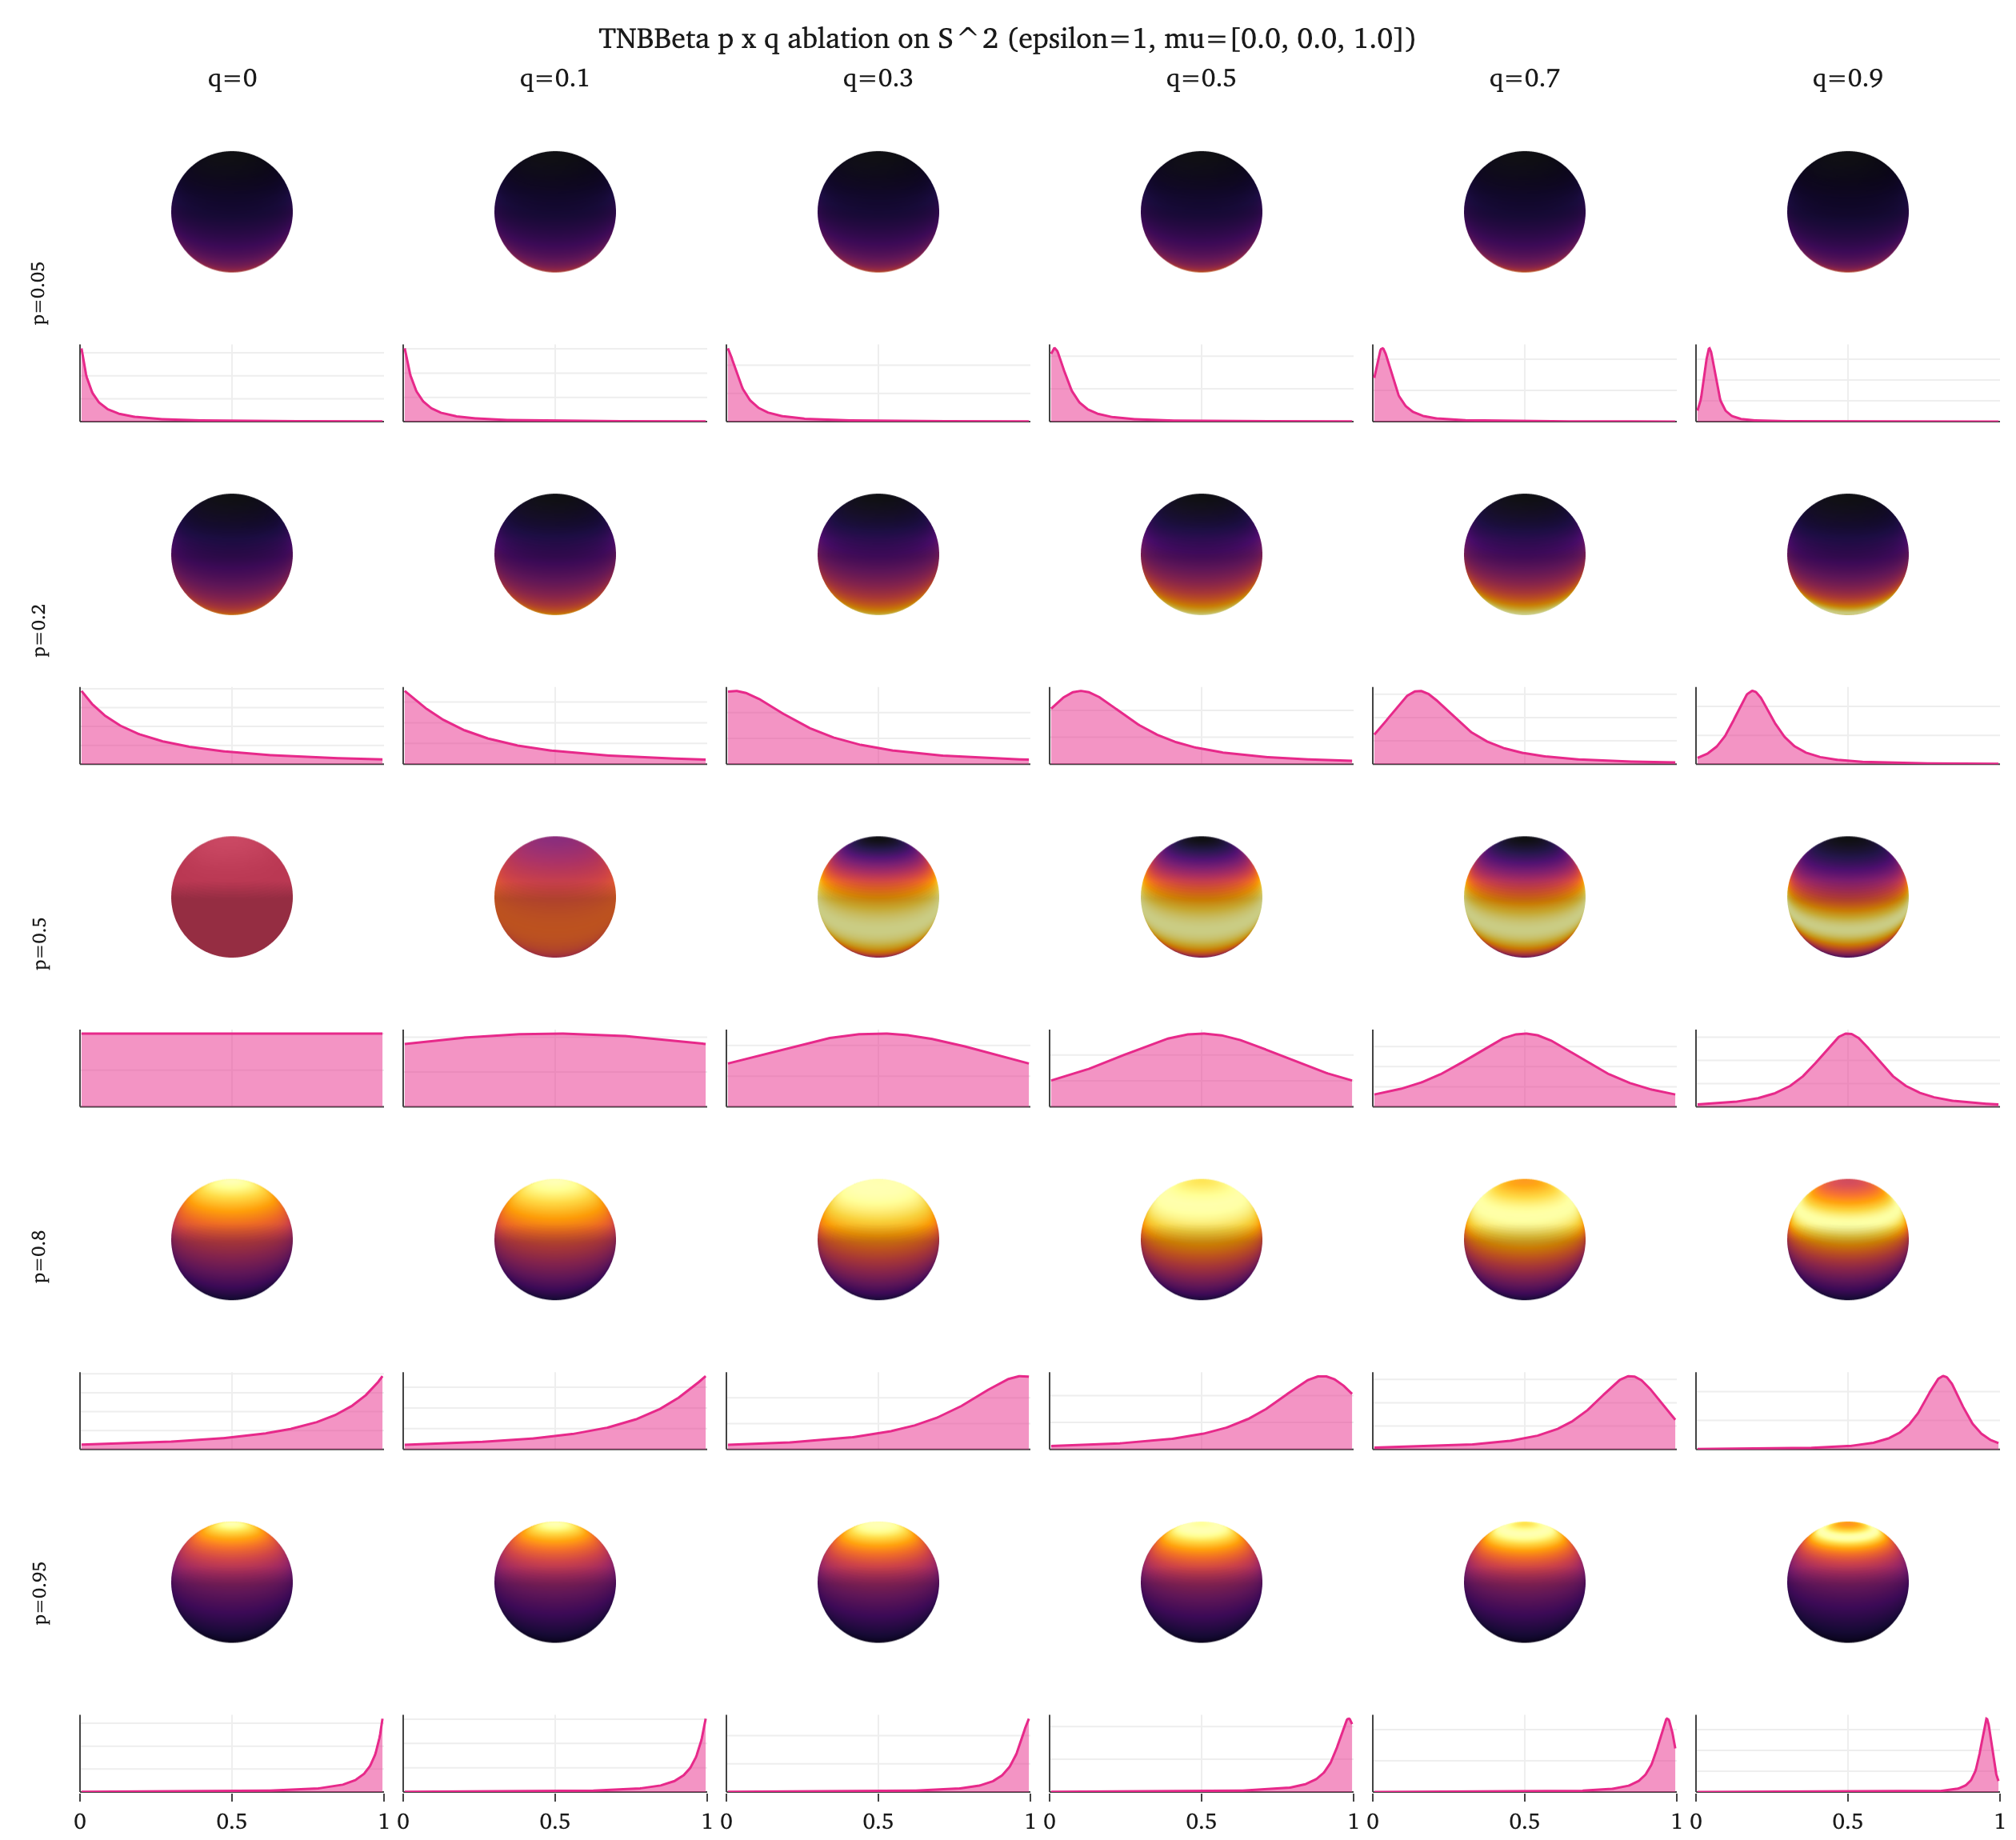
\includegraphics[width=\linewidth]{assets/pq_ablation.png}
        \caption{$p \times q$ ablation ($\varepsilon = 1$).}
        \label{fig:pq-ablation}
    \end{subfigure}
    \hfill
    \begin{subfigure}[t]{0.49\textwidth}
        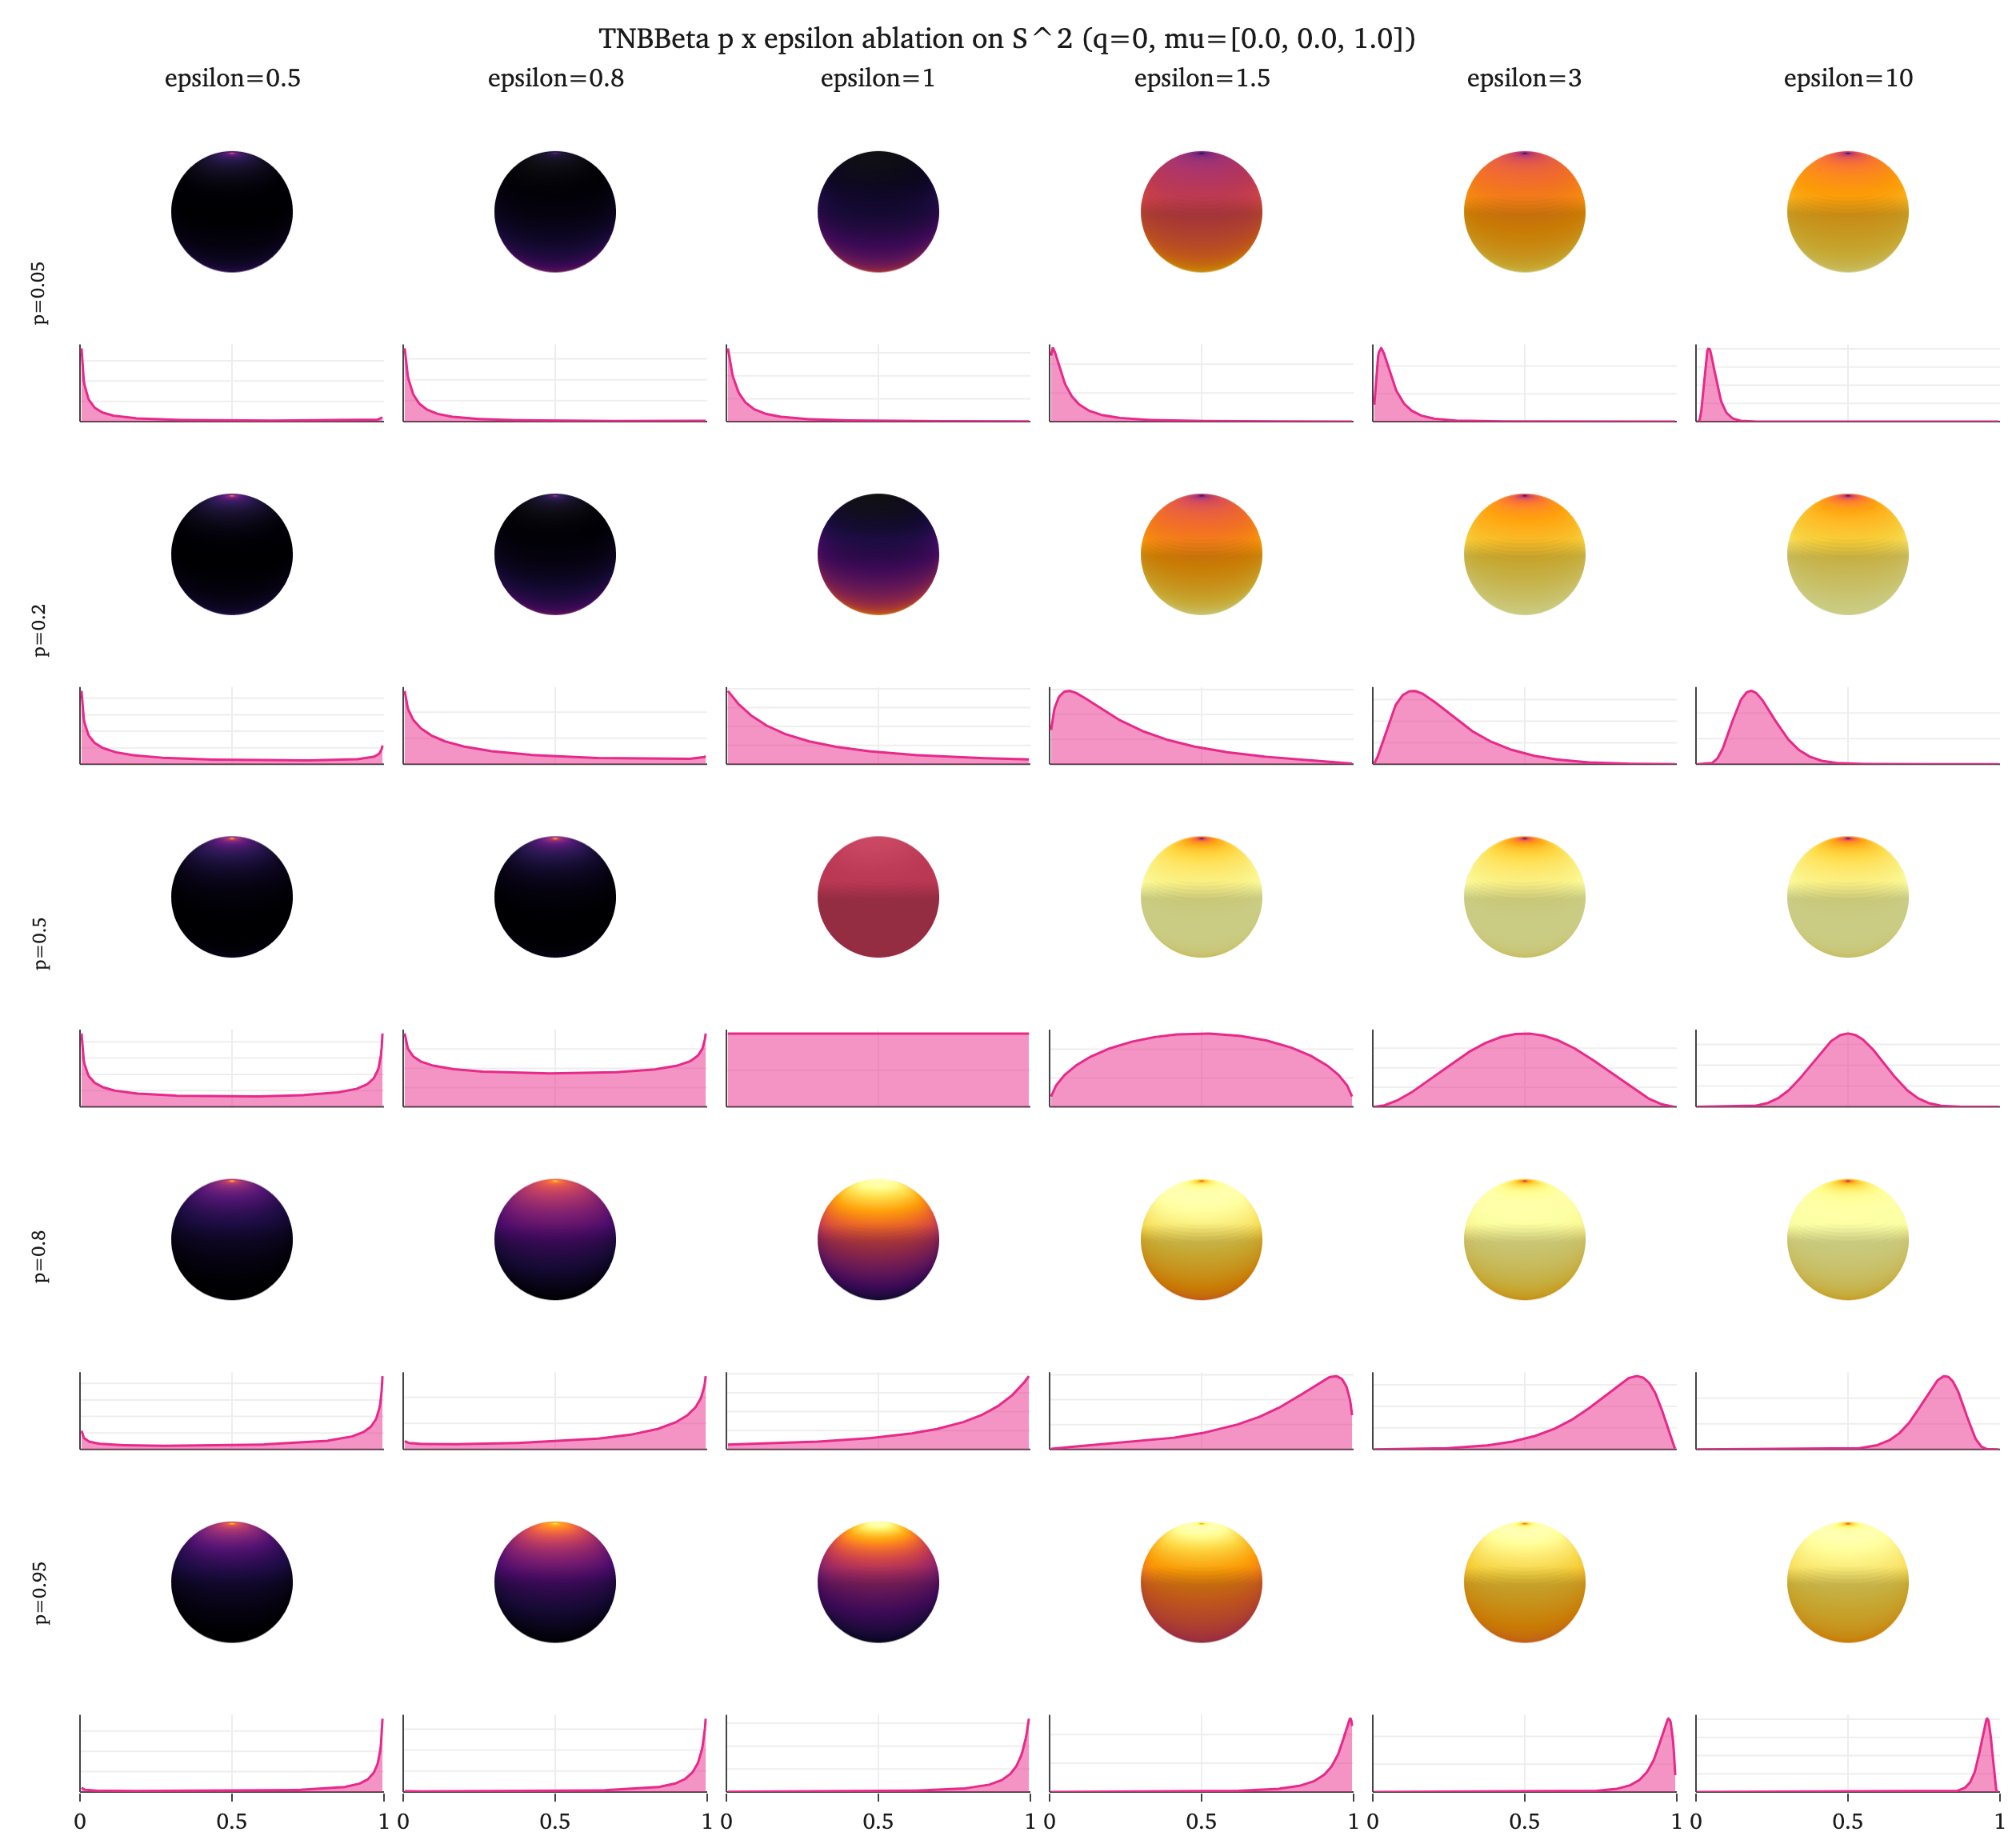
\includegraphics[width=\linewidth]{assets/p_epsilon_ablation.png}
        \caption{$p \times \varepsilon$ ablation ($q = 0$).}
        \label{fig:p-epsilon-ablation}
    \end{subfigure}
    \caption{TNBBetaSpherical on $S^2$ ($\mu = [0, 0, 1]$): each cell shows the
    spherical log-density above its corresponding univariate density on $(0, 1)$.}
    \label{fig:ablations}
\end{figure}
